\chapter{Estado del Arte}
\label{chapter:estadoarte}


El objetivo de este apartado es hacer un recorrido por el estado del arte relacionado con el proyecto, este recorrido lo enfocaremos desde tres puntos de vista diferentes:
\begin{itemize}
	\item \textbf{Procesamiento del Lenguaje Natural}: En la sección \ref{section:arte:pln}  nos centraremos en el procesamiento del lenguaje natural y su evolución a lo largo del tiempo. 
	\item \textbf{\textit{Deep Learning} y aplicación al Procesamiento del Lenguaje Natural}: En la sección \ref{section:arte:deep}  pondremos foco en el \textit{Deep Learning}, sus ventajas y cómo se están aplicando estos métodos al procesamiento del lenguaje natural. 
	\item \textbf{\textit{Big Data} y \textit{Fast Data}}: Por último, en la sección \ref{section:arte:big}, haremos un repaso a la evolución del \textit{Big Data} y cómo la tendencia actual es realizar el procesamiento en tiempo real mediante \textit{Fast Data}.
\end{itemize}

Por último, una vez analizados los diferentes puntos de vista, en la sección \ref{section:arte:ant} enumeraremos trabajos anteriores relacionados con nuestro proyecto. Estos trabajos nos serán de utilidad para justificar la realización de nuestro proyecto y su viabilidad. 

\section{Procesamiento de lenguaje natural}
\label{section:arte:pln}

\subsection{Historia}

Para hablar de los orígenes del Procesamiento del Lenguaje Natural (a partir de ahora se usarán indistintamente las siglas PLN) tal y como lo conocemos, tendríamos que remontarnos a los años 50, concretamente al artículo ``\textit{Computing Machinery and Intelligence}'' escrito por Alan Turing \cite{turing_1950}. En este artículo aparece el PLN dentro del campo de la inteligencia artificial y se presenta por primera vez el conocido ``Test de Turing`''. Este test convirtió la pregunta abstracta de ``¿Son capaces de pensar las máquinas?'' en un juego llamado: ``\textit{The Imitation Game}''. El juego propuesto inicialmente, de forma muy resumida, consiste en ver si una persona (interrogador) interrogando a dos personas (un hombre y una mujer), era capaz de descubrir el sexo de cada una; la modificación del mismo sustituye las dos personas de distinto sexo por una persona y una máquina y el interrogador debe ser capaz de descubrir si las preguntas están siendo respondidas por un humano o una máquina. En el caso de que no sepa discernir, la computadora gana la partida. Podemos encontrar más información al respecto en el libro \cite{turing}.



A partir de los avances de Turing y hasta los años 80 el crecimiento en el campo del PLN se produjo principalmente con la creación de complejos sistemas basados en reglas escritas a mano. Fue en esta década cuando empezamos a vivir la incorporación de algoritmos de \textit{Machine Learning} enfocados al procesamiento del lenguaje natural. Este hecho se vio motivado principalmente por el increíble avance en la capacidad de cómputo, ya predicho por la ley de Moore, y por la aplicación de teorías ya existentes como los trabajos de Chomsky. 


Desde el comienzo de la aplicación de modelos de \textit{Machine Learning}, y de nuevo motivados por el crecimiento de la capacidad computacional de los sistemas actuales, se ha pasado de utilizar árboles de decisión, que creaban de manera automática reglas similares a las que se venían creando manualmente, a los modelos de \textit{deep learning} que están en auge en la última década. 

\subsection{Aplicaciones}

En el apartado anterior hicimos referencia a ``\textit{The Imitation Game}'' como inicio de lo que hoy conocemos como procesamiento del lenguaje natural, sin embargo, las aplicaciones en este campo han crecido de forma vertiginosa en estos 70 años, principalmente en las últimas décadas. Hoy en día, si tuviéramos que contestar a la pregunta: ``¿son capaces de pensar las máquinas?'', implicaría algo más que superar el test de Turing. Mirando a nuestro alrededor nos encontraríamos con asistentes de voz como Alexa o Siri que, no solo contestan a nuestras preguntas, si no que realizan un trabajo de pasar nuestra voz a texto (\textit{Speech to Text}) y de nuevo el texto resultante a voz (\textit{Text to Speech}). Nos encontraríamos también con sistemas capaces de realizar traducciones simultáneas, otros capaces de autocompletar textos, de identificar preguntas y respuestas, de clasificar textos de acuerdo a temas o autores, incluso de analizar sentimientos positivos o negativos teniendo como entrada un texto u opinión.


Según \cite{goldberg_2017} todos estos problemas tan diversos podríamos clasificarlos según en el punto del análisis que nos centremos: 

\begin{itemize}
	\item \textbf{Análisis de palabras}: En este tipo de problemas se pone foco en las palabras, como pueden ser ``perro'', ``hablar'', ``piedra'' y necesitamos decir algo sobre ellas. Por ejemplo: ``¿estamos hablando de un ser vivo?'', ``¿a qué lenguaje pertenece?'', ``¿cuáles son sus sinónimos o antónimos?''. Actualmente este tipo de problemas son menos frecuentes, ya que normalmente no pretendemos analizar palabras aisladas sino que es preferible basarse en un contexto. 
	
	\item \textbf{Análisis de textos}:  En este tipo de problemas no trabajamos solo con palabras aisladas, sino que disponemos de una pieza de texto que puede ser una frase, un párrafo o un documento completo y tenemos que decir algo sobre él. Por ejemplo: ``¿se trata de spam?'', ``¿qué tipo de texto es?'', ``¿el tono es positivo o negativo?'', ``¿quién es su autor?''. Este tipo de problemas son muy comunes y nos vamos a referir a ellos como \textbf{problemas de clasificación de documentos}.   
	
	\item \textbf{Análisis de textos pareados}: En esta clase de análisis disponemos de  dos textos (también podrían ser palabras aisladas) y tenemos que decir algo sobre ellos. Por ejemplo, ``¿los textos son del mismo autor?'', ``¿son pregunta y respuesta?'', ``¿son sinónimos?'' (para el caso de palabras aisladas).
	
	\item \textbf{Análisis de palabras en contexto}: En estos casos de uso, a diferencia del primer análisis que trataba unicamente con  palabras aisladas, tenemos que clasificar una palabra en particular en función del contexto en el que se encuentra. 
	
	\item \textbf{Análisis de relación entre palabras}: Este último tipo de análisis tiene como objetivo deducir la relación entre dos palabras existentes en un documento. 
	
\end{itemize}

Dependiendo del problema que queramos abordar usaremos un tipo de características del lenguaje u otro, por ejemplo, es usual que si estamos analizando palabras aisladas nos centremos en las letras de una palabra, sus prefijos o sufijos, su longitud, la información léxica extraída de diccionarios como \textit{WordNet} \cite{wordnet}, etc. En cambio, si estamos trabajando con texto, lo normal es que nos fijemos en otros conceptos estadísticos como el histograma de las palabras dentro del texto, ratio de palabras cortas vs largas, número de veces que aparece una palabra en un texto comparado con el resto de textos, etc.

El proyecto que se presenta en este documento está centrado en el análisis de textos, concretamente en extraer los temas de un documento (o llamada). Este tipo de problemas se conoce como modelización de \textit{topics}. 

En el siguiente punto de este apartado nos centraremos en algunos modelos y avances en este área que puedan servirnos de apoyo para nuestro proyecto. 


\subsection{Modelización de temas}
La modelización de topics hace referencia a un grupo de algoritmos de \textit{Machine Learning} que infieren la estructura latente existente en un grupo de documentos. 

Aunque la mayoría de los algoritmos de modelización son no supervisados, al igual que los algoritmos tradicionales de \textit{clustering}, existen también algunas variantes supervisadas que necesitan disponer de documentos etiquetados. 

Quizás el algoritmo más conocido para la modelización de topics sea el \textit{Latent Dirichlet Allocation} (normalmente conocido por su acrónimo, LDA). LDA fué presentado en 2003 en el artículo \cite{Blei_LDA}. Este algoritmo no supervisado asume que cada documento es una distribución probabilística de \textit{topics} y cada \textit{topic}, a su vez, es una distribución de palabras del documento. LDA usa una aproximación llamada ``\textit{bag of words}'', en la que cada documento es tratado como un vector con el conteo de las palabras que aparecen en el mismo. La principal característica de LDA es que la colección de documentos comparten los mismos topics, pero cada documento contiene esos topics en una proporción diferente. 


A partir de LDA surgieron numerosas variantes que repasaremos de forma breve, por ejemplo, en el mismo año de la creación de LDA y también presentado por los mismos autores en \cite{Blei_HTM}, surgió una \textbf{variante jerárquica} que permitía representar los \textit{topics} jerárquicamente. En 2006 en \cite{Blei_DTM} se desarrolla un modelo LDA dinámico denominado DTM (\textit{Dinamic Topic Model}), en el que se introduce la variable temporal y los \textit{topics} pueden ir cambiando a lo largo del tiempo. En el artículo \cite{Blei_CTM} nos encontramos con otra variante de LDA llamada CTM (\textit{Correlated topic model}) que nos permite encontrar correlaciones entre \textit{topics}, ya que algunos temas es probable que sean más similares entre sí. Por último, nos encontramos con una variante de LDA denominada ATM (\textit{Author-Topic Model}) propuesta  por	Michal Rosen-Zvi en su artículo \cite{Rosen-Zvi_AMA_2010}  y desarrollada por el mismo en 2010, en la que los documentos son una distribución probabilística tanto de autores como de \textit{topics}.    


Podemos encontrar un resumen más completo del estado del arte en cuanto a la modelización de \textit{topics} en el artículo \cite{Mahmood2013LiteratureSO}. 

\section{Deep Learning  y aplicación al PLN}
\label{section:arte:deep}

El objetivo de esta sesión es entender el concepto de \textit{Deep Learning} y analizar el estado del arte del \textit{Deep Learning} aplicado al Procesamiento del Lenguaje Natural. Para poder entender el \textit{Deep Learning} es conveniente entender los modelos de aprendizaje supervisados y saber qué provoca su aparición y popularidad de los últimos años. Posteriormente nos centraremos en los fundamentos del \textit{Deep Learning} y cómo es utilizado en la representación de palabras. Por último, comentaremos algunas arquitecturas especializadas y su aplicación en el ámbito del Procesamiento del Lenguaje Natural.


\subsection{Aprendizaje supervisado}
El aprendizaje supervisado consiste en aprender una función a través de un conjunto de datos llamados de entrenamiento, mediante la cual podamos obtener una salida a partir de una determinada entrada. Se espera que esta función, una vez realizado el entrenamiento, sea capaz de producir una salida correcta incluso para datos nunca vistos. Es muy habitual el uso de estos tipos de algoritmos para casos de clasificación y/o predicción. 

Buscar entre todas las posibles infinitas funciones para encontrar la que mejor se adapte a nuestro conjunto de datos es un trabajo inviable, es por ello que normalmente se realiza la búsqueda entre un conjunto de funciones limitadas. En un primer lugar, y hasta hace aproximadamente una década, los modelos más populares de aprendizaje supervisado fueron los modelos lineales, provenientes del mundo de la estadística, estos modelos son fáciles de entrenar, fáciles de interpretar y muy efectivos en la práctica. 

A partir de entonces, y motivado en parte por el aumento en las capacidades de cómputo, surgen otros modelos como las máquinas de vectores de soportes (\textit{Support Vector Machines}, SVMs) o las redes neuronales, en las que nos centraremos en el siguiente apartado.


\subsection{Deep Learning}
Dentro del \textit{Machine Learning} y usualmente relacionado con el aprendizaje supervisado, nos encontramos con un sub-campo denominado \textbf{Deep Learning} que utiliza las redes neuronales para la creación de modelos. 

Como su nombre indica las redes neuronales consisten en unidades de cómputo llamadas neuronas que están interconectadas entre sí. Una neurona es una unidad de cómputo que posee múltiples  entradas y una  salida, esta neurona multiplica cada entrada por un peso para posteriormente realizar una suma y, por último, aplicar una función de salida no lineal. Si los pesos se establecen correctamente y tenemos un número suficiente de neuronas, una red neuronal puede aproximar a un conjunto muy amplio de funciones matemáticas. 

En las redes neuronales, las neuronas suelen organizarse por capas que se encuentran conectadas entre sí. Mientras más capas tengamos, más características podremos extraer de nuestros datos de entrada y podremos aproximar un mayor número de funciones (sin perder de vista el sobrentrenamiento). 


El primero y más simple de los tipos de redes neuronales es el denominado \textit{Feed Forward Neural Network} (\textbf{FFNN}), este tipo de redes recibe este nombre porque no existen ciclos entre sus neuronas y las conexiones se realizan siempre desde las capas anteriores a las capas posteriores. 


Una de las arquitectura más comunes de FFNN es el preceptrón multicapa (en inglés multilayer perceptron o \textbf{MLP}). Esta arquitectura contiene tres o más capas de neuronas totalmente conectadas, es decir, la salida de una neurona de una capa se encuentra conectada a la entrada de todas las neuronas de la siguiente capa. Las capas de una arquitectura MLP son:

\begin{itemize}
	\item \textbf{Capa de entrada}: Se trata de la capa en la que introduciremos los datos en la red. Esta capa carece de procesamiento.
	\item \textbf{Capas ocultas}: Son las capas intermedias, cuyo número puede variar, tienen como entrada la salida de las neuronas de la capa anterior y su salida alimenta a las neuronas de la capa posterior.  
	\item \textbf{Capa de salida}: Los valores de salida de las neuronas de esta capa se corresponden con la salida de la red.
\end{itemize}
 
\begin{figure}[!ht]
	\centering
	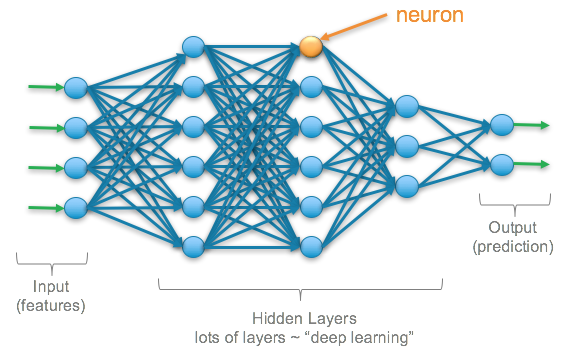
\includegraphics[width=0.68\textwidth]{images/arte/mlp}
	\caption{Ejemplo de arquitectura MLP. Fuente \cite{mlp}}
	\label{fig:mlp}
\end{figure}



Hablamos que una red es profunda cuando contiene un gran número de capas, por ello el término de \textit{Deep Learning}. En la Figura \ref{fig:mlp} observamos un ejemplo de arquitectura MLP y como la denominamos \textit{Deep Learning} al crecer el número de capas ocultas.


\subsection{Representación de palabras en PLN}% Podemos llamarle embedding o representación de palabras

Es usual, en el ámbito del reconocimiento de imágenes, utilizar información acerca de la dimensionalidad de las mismas. Este tipo de información nos permite extraer características  teniendo en cuenta los píxeles vecinos. Tradicionalmente, en el ámbito del Procesamiento del Lenguaje Natural, esto no se ha llevado a cabo debido a que cada palabra (o n-grama) se trataba como una entidad aislada utilizando una codificación de las palabras denominada \textbf{one-hot encoding}. 

En cambio, existe otro método de representar las palabras en el lenguaje natural que sí es capaz de captar la ``dimensionalidad'' de una forma similar a como lo realizamos en las imágenes. Este modo, conocido como \textit{\textbf{word embedding}}, deja de tratar la palabra como un ente aislado y  es capaz de captar el significado de la misma, esta representación se denomina distribuida y consiste en convertir las palabras en vectores en los que cada dimensión capte características diferentes de las palabras. Este tipo de representaciones dará lugar a vectores similares para palabras semánticamente parecidas. 


\begin{figure}[!ht]
	\centering
	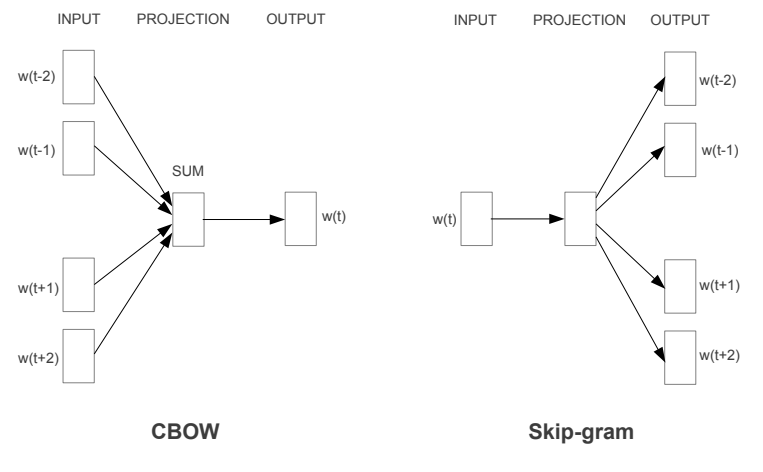
\includegraphics[width=0.7\textwidth]{images/arte/word2vec}
	\caption{Arquitecturas CBOW y Skip-gram. Fuente \cite{word2vec}}
	\label{fig:wor2vec}
\end{figure}

Una de las soluciones más populares que nos permiten convertir una palabra a un vector (\textit{word2vec}) que contenga información de la palabra en función del contexto se detallan en el artículo \cite{word2vec} . Aquí se presentaron dos modelos llamados \textbf{Skip-Gram} y \textbf{CBOW} cuya arquitectura podemos ver en la Figura \ref{fig:wor2vec}. Estos modelos utilizan redes neuronales para predecir una palabra en función de su contexto o el contexto en función de una palabra, el vector que se utiliza para representar la palabra es el vector de pesos de la capa oculta. 



\subsection{Arquitecturas especializadas}

Después de introducir las redes neuronales y el modo en el que podemos representar las palabras, frases o documentos para ser usados como entrada en nuestro modelo; vamos a centrarnos en comentar dos tipos de redes neuronales que se usan de manera tradicional en tareas de Procesamiento de Lenguaje Natural. 

Los dos tipos de redes neuronales que comentaremos son las redes neuronales convolucionales y las redes neuronales recurrentes. Haremos una introducción a cada una de ellas, comentaremos sus aplicaciones al PLN y sus ventajas e inconvenientes con respecto a otro tipo de métodos. 


\subsubsection{Redes neuronales convolucionales}

Las redes neuronales convolucionales (llamadas usualmente CNN, por su nombre en inglés \textit{\textbf{C}onvolutional \textbf{N}eural \textbf{N}etworks}) son un tipo de redes neuronales que deben su nombre a la operación matemática de convolución que realizan. Esta operación consiste en aplicar a una matriz de entrada multidimensional, un filtro o kernel también multidimensional y obtener una salida, también denominada mapa de características. En la Figura \ref{fig:cnn1} podemos ver una representación gráfica de esta operación para un ejemplo de 2 dimensiones. 

\begin{figure}[!ht]
	\centering
	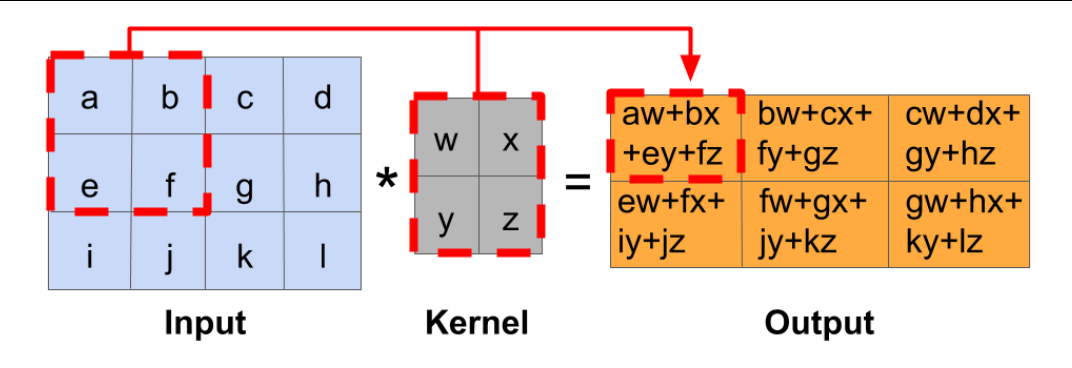
\includegraphics[width=0.7\textwidth]{images/arte/cnn1}
	\caption{Ejemplo de una convolución de dos dimensiones. Fuente \cite{temariodeeplearning}}
	\label{fig:cnn1}
\end{figure}

Es usual en las redes convolucionales  utilizar diferentes kernels sobre una misma entrada, obteniendo diferentes salidas que permitan reconocer distintos patrones. Los pesos del kernel junto con el sesgo, son los parámetros que serán necesarios calcular en el entrenamiento y en el caso de las redes convolucionales, se denominan mapas de características.

Aunque la convolución simple que comentamos es la operación básica en las redes convolucionales, es usual añadirle algunas variantes (o configurarla con algunos parámetros) que nos permitan variar la dimensión de salida una vez hemos aplicado la convolución; algunas de estas variaciones más comunes son el \textbf{\textit{zero padding}} y la \textbf{convolución por pasos}.

\begin{figure}[!ht]
	\centering
	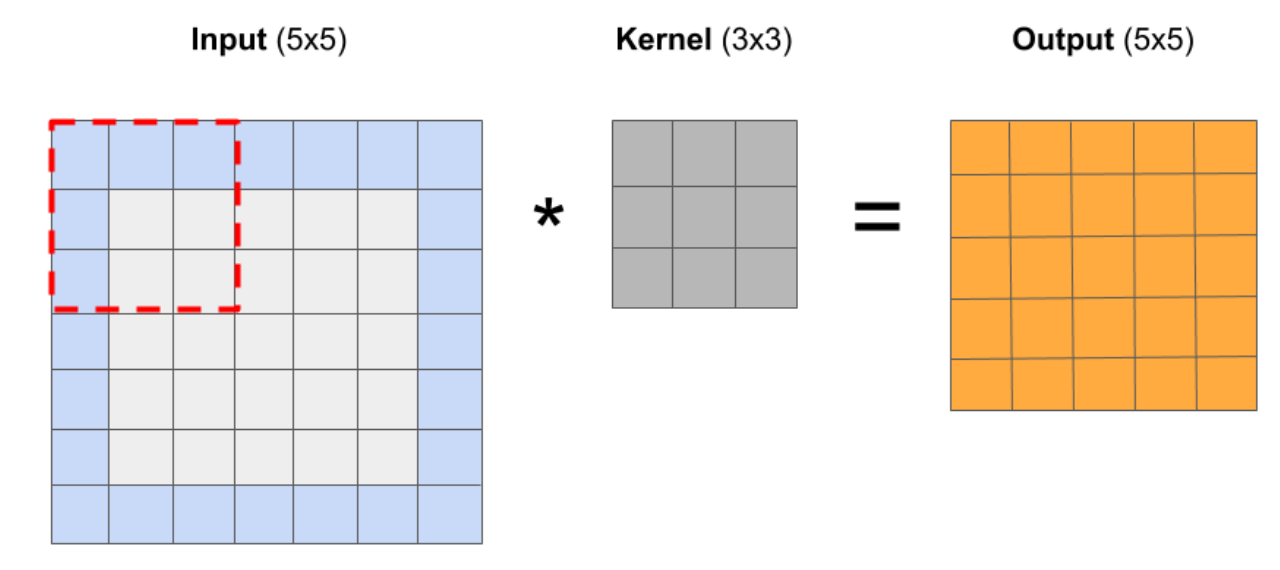
\includegraphics[width=0.7\textwidth]{images/arte/padding}
	\caption{Ejemplo de aplicación de \textit{zero padding} para mantener la dimensionalidad. Fuente \cite{temariodeeplearning}}
	\label{fig:padding}
\end{figure}

Como observamos en la Figura \ref{fig:cnn1}, al aplicar el kernel a los datos de  entrada estamos reduciendo la dimensionalidad de la salida. A menudo es posible que esto no nos interese y queramos mantener la dimensionalidad en la salida; para ello recurrimos a un método denominado \textit{zero padding} que consiste en añadir '0s' en los bordes de nuestra entrada con el objetivo de preservar la dimensionalidad en la salida. En la Figura \ref{fig:padding} podemos ver un ejemplo de aplicación de \textit{zero padding}.




Por otro lado, es también posible que queramos reducir aún más la dimensión de salida, principalmente por un tema de eficiencia y reducción de los tiempos de ejecución, a costa de perder información de algunas características en la salida. Para ello podemos utilizar la convolución por pasos (o \textit{strided} por su nombre en inglés). Este método consiste en aplicar el kernel realizando saltos en lugar de hacerlo sobre celdas consecutivas,  tal y como podemos ver en la Figura \ref{fig:strided}.

\begin{figure}[!ht]
	\centering
	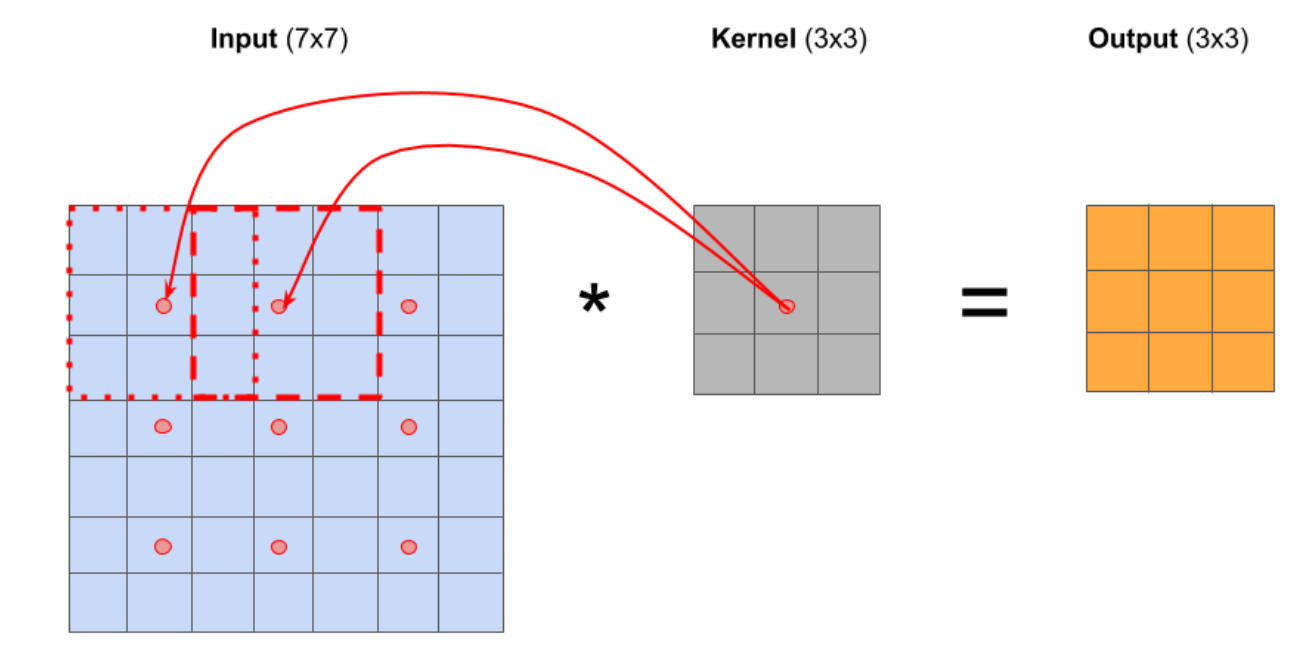
\includegraphics[width=0.7\textwidth]{images/arte/strided}
	\caption{Ejemplo de aplicación de convolución por pasos para reducir la dimensionalidad. Fuente \cite{temariodeeplearning}}
	\label{fig:strided}
\end{figure}



El proceso explicado anteriormente correspondería con una capa convolucional, que son el corazón de las redes neuronales convolucionales, sin embargo, en una red neuronal convolucional estas capas coexisten con otro tipo de capas que nos ayudaran a mejorar nuestros modelos. Las más usuales son:

\begin{itemize}
	\item Capa de agrupamiento (\textit{polling} en inglés): El objetivo de esta capa es agrupar un conjunto de salidas para obtener un único valor. Al conjunto de valores de entrada (seleccionado de nuevo con un filtro) se le aplica una función para obtener un único valor. Aunque se pueden utilizar diferentes funciones, como puede ser la media, lo más usual es aplicar la función de máximo (\textit{max-polling}). Es habitual, intuir que usando esta función nos estamos quedando con las características más relevantes de cada cuadrante (del tamaño del filtro) de la entrada. En la Figura \ref{fig:pooling} podemos ver un ejemplo de agrupamiento utilizando la función de máximo. 
	\item Capa totalmente conectada: Hemos visto ejemplos de capas totalmente conectadas al introducir las redes neuronales, esta capas usualmente se usan al final de nuestra red para tareas de clasificación, teniendo la última capa un número de neuronas igual al número de clases que pretendemos clasificar. 
	\item Capa RELU: Si observamos la descripción de la operación de convolución nos damos cuenta de que se trata de una operación totalmente lineal, es por ello que después de cada capa de convolución es usual agregar una capa no lineal (también llamada capa de activación). Aunque se pueden utilizar otras funciones como la tangente o la función sigmoide, lo más usual es utilizar la función RELU.
	
	\item Capa de Dropout: Esta capa tiene como funcionalidad prevenir el sobreentrenamiento en las redes neuronales, desactivando un número aleatorio de entradas de la capa, forzando a la red a ser redundante y permitiendo dar una clasificación correcta sin tener todas las entradas activas. 
	
\end{itemize}

\begin{figure}[!ht]
	\centering
	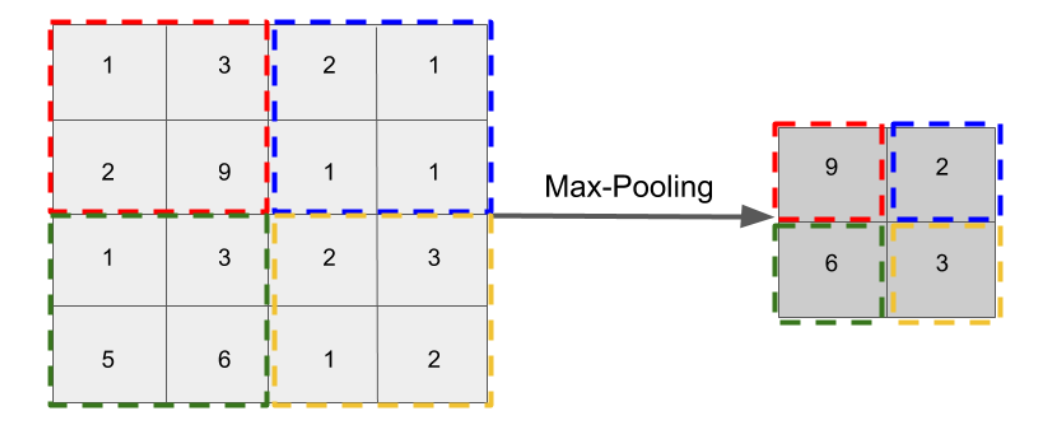
\includegraphics[width=0.7\textwidth]{images/arte/pooling}
	\caption{Ejemplo de aplicación de \textit{max-pooling}. Fuente \cite{temariodeeplearning}}
	\label{fig:pooling}
\end{figure}


Tras esta visión general sobre las redes neuronales generales, podemos enumerar las ventajas que conllevan: 

\begin{itemize}
	\item Por un lado, aunque no hemos entrado en detalles sobre el proceso de entrenamiento de las redes convolucionales, se puede intuir que el aplicar un mismo kernel sobre toda la entrada provoca que el número de parámetros a aprender (los valores del kernel) con respecto a una red totalmente conectada será mucho menor. Esto provoca una \textbf{reducción del tiempo de entrenamiento necesario}. 
	\item Por otro lado, el hecho de compartir el kernel provoca que podamos \textbf{capturar una misma característica en la entrada a pesar de su traslación}. Por ejemplo, si estamos detectando un objeto en una imagen un modelo convolucional podrá detectar ese objeto a pesar de su movimiento por la imagen. 
\end{itemize}


\begin{figure}[!ht]
	\centering
	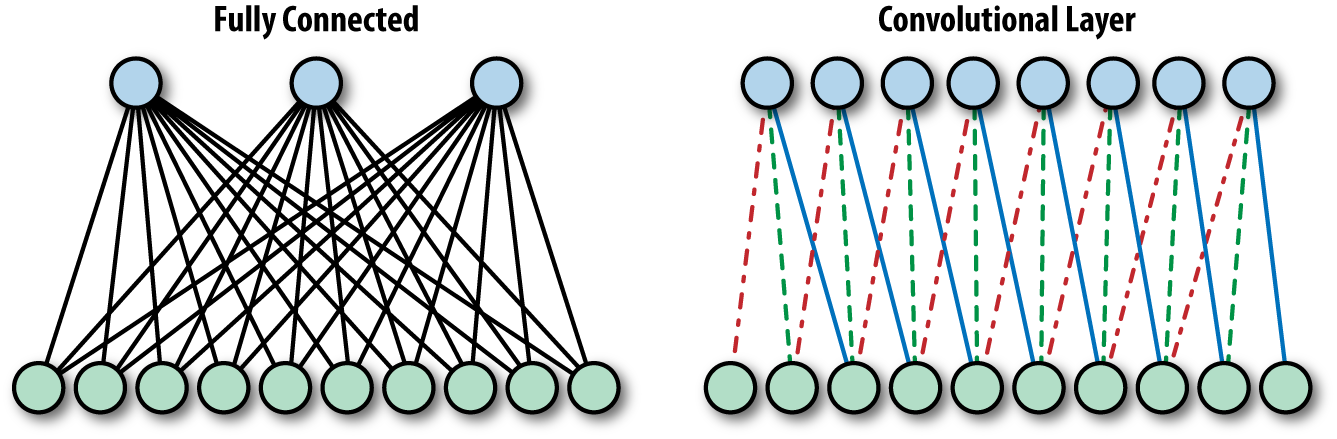
\includegraphics[width=0.7\textwidth]{images/arte/traditionalvscnn}
	\caption{Comparación capa tradicional totalmente conectada con capa convolucional. Fuente \cite{hope_lieder_resheff_2017}}
	\label{fig:tradvscnn}
\end{figure}



Sin embargo, las redes neuronales convolucionales deben usarse en datos que contengan coherencia local ya que esa es su fortaleza. \textbf{En datos sin coherencia local las redes neuronales convolucionales no lograrían obtener un buen rendimiento} como las redes neuronales tradicionales vistas anteriormente. Si observamos la Figura \ref{fig:tradvscnn} podemos ver la diferencia entre las capas de ambos tipos de redes y cómo la capa convolucional se centra más en las estructuras locales.




Encontramos una explicación más profunda sobre las redes convolucionales y su uso general en \cite{temariodeeplearning}. Aunque, como podemos imaginar, el uso más extendido de este tipo de redes es para el tratamiento de imágenes, nosotros nos centraremos en tener una breve visión de su aplicación al Procesamiento del Lenguaje Natural, que también puede ampliarse en \cite{goldberg_2017}.



Al aplicar las redes tradicionales al PLN, solemos ignorar el orden en el que las palabras aparecen en las frases, o las frases en el documento, siguiendo una aproximación CBOW;  esto suele ser problemático a la hora de realizar, por ejemplo, un análisis de sentimientos ya que no es lo mismo encontrar la palabra ``malo'' aislada que el bigrama ``no malo''. Aunque el uso de bi-gramas y N-gramas de mayor orden puede mejorar esta situación el coste puede volverse inasumible. 

Es en este ámbito dónde las redes neuronales convolucionales pueden ser de gran ayuda, ya que gracias a la capacidad comentada para detectar estructuras locales serían capaces de identificar estos N-gramas de forma automática para ser usados posteriormente en tareas predictivas. 




\subsubsection{Redes neuronales recurrentes}
Otro de los modelos usualmente usados en tareas de Procesamiento del Lenguaje Natural son las redes neuronales recurrentes, (llamadas usualmente RNN, por su nombre en inglés \textit{\textbf{R}ecurrent \textbf{N}eural \textbf{N}etworks}). Hasta ahora todos los modelos de redes neuronales que hemos citado funcionaban siempre en una dirección, las neuronas de una capa anterior producían una salida que era la encargada de activar las neuronas de la capa posterior. En las redes recurrentes veremos que las salidas de una neurona en una capa posterior pueden tener una conexión con una neurona de una capa anterior. Esto crea una especie de \textbf{memoria} que nos permite modificar la respuesta de la red en función de los datos que se hayan procesado anteriormente (incluso reaccionar con datos que lleguen posteriormente).

\begin{figure}[!ht]
	\centering
	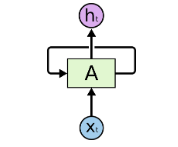
\includegraphics[width=0.32\textwidth]{images/arte/rnn}
	\caption{Ejemplo RNN. Fuente \cite{colahblog}}
	\label{fig:rnn}
\end{figure}

Las conexiones en una red neuronal recurrente pueden tener muchas variaciones por lo que es usual hablar del concepto de \textbf{celda}. Una celda suele tener como entrada los valores de la secuencia y el estado de la red neuronal en el paso anterior; y como salida la respuesta de la red neuronal a dicha entrada y el estado de la red neuronal en el paso actual. 



En la Figura \ref{fig:rnn} observamos un ejemplo de red neuronal recurrente en el que tenemos como entrada el valor de la secuencia $x_{t}$ y el estado de la red en el paso anterior (conexión en bucle). Producimos una respuesta $h_{t}$ y un estado (conexión en bucle). Sin embargo, posiblemente esta representación sea algo más confusa para comprender su funcionamiento que si procedemos a ``desenrollar'' la red neuronal haciéndola más similar a los modelos vistos hasta ahora. En la Figura \ref{fig:rnn2} podemos ver el resultado de ``desenrollar'' la red; hay que tener en cuenta con esta representación que los parámetros usados por cada celda son exactamente los mismos.

\begin{figure}[!ht]
	\centering
	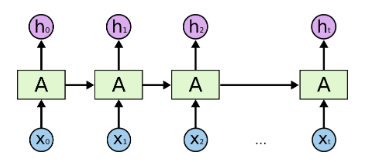
\includegraphics[width=0.65\textwidth]{images/arte/rnn2}
	\caption{Ejemplo RNN ``desenrollada''. Fuente \cite{colahblog}}
	\label{fig:rnn2}
\end{figure}



Aunque no entraremos en detalles sobre el entrenamiento de redes neuronales, es importante saber que existen dos problemas diferentes provocados ambos por usar los mismos parámetros en todas las celdas que provocan la inestabilidad durante el proceso de entrenamiento. Estos problemas son la \textbf{desaparición del gradiente}, que ocurre al multiplicar el gradiente consigo mismo múltiples veces cuando este es menor que 1, y la \textbf{explosión del gradiente}, que ocurre por el mismo motivo cuando este es mayor que 1. 

Para mitigar estos problemas es importante el diseño de las celdas, a continuación veremos de manera resumida los dos tipos de celdas más usados en las redes neuronales recurrentes. Las celdas que comentaremos están compuestas por diferentes mecanismos internos, denominados puertas, que gestionan el flujo de información a lo largo de la misma. 


El primer tipo de celdas  son las celdas \textit{Long Short Term Memory} (\textbf{LSTM}). Este tipo de celdas se comportan bien en situaciones que queremos encontrar patrones entre registros que se encuentran separados en la secuencia, esto es algo muy usual, por ejemplo, en el caso de PLN cuando en una misma frase una palabra hace referencia a otra que apareció a una distancia de varias palabras. 
	
Para conseguir este objetivo, parece evidente que es importante controlar la memoria en cada una de las celdas. Una celda LSTM realiza esta tarea con las siguientes puertas: 
	\begin{itemize}
		\item Puerta de entrada: Controla que información se añade a la memoria de la red. 
		\item Puerta de olvido: Controla, a partir de la memoria del paso anterior y de la entrada, qué información debe conservarse en la memoria. 
		\item Puerta de salida:  Es la encargada de calcular la salida de la red, $h_{t}$, en el paso actual. 
	\end{itemize}

\begin{figure}[!ht]
	\centering
	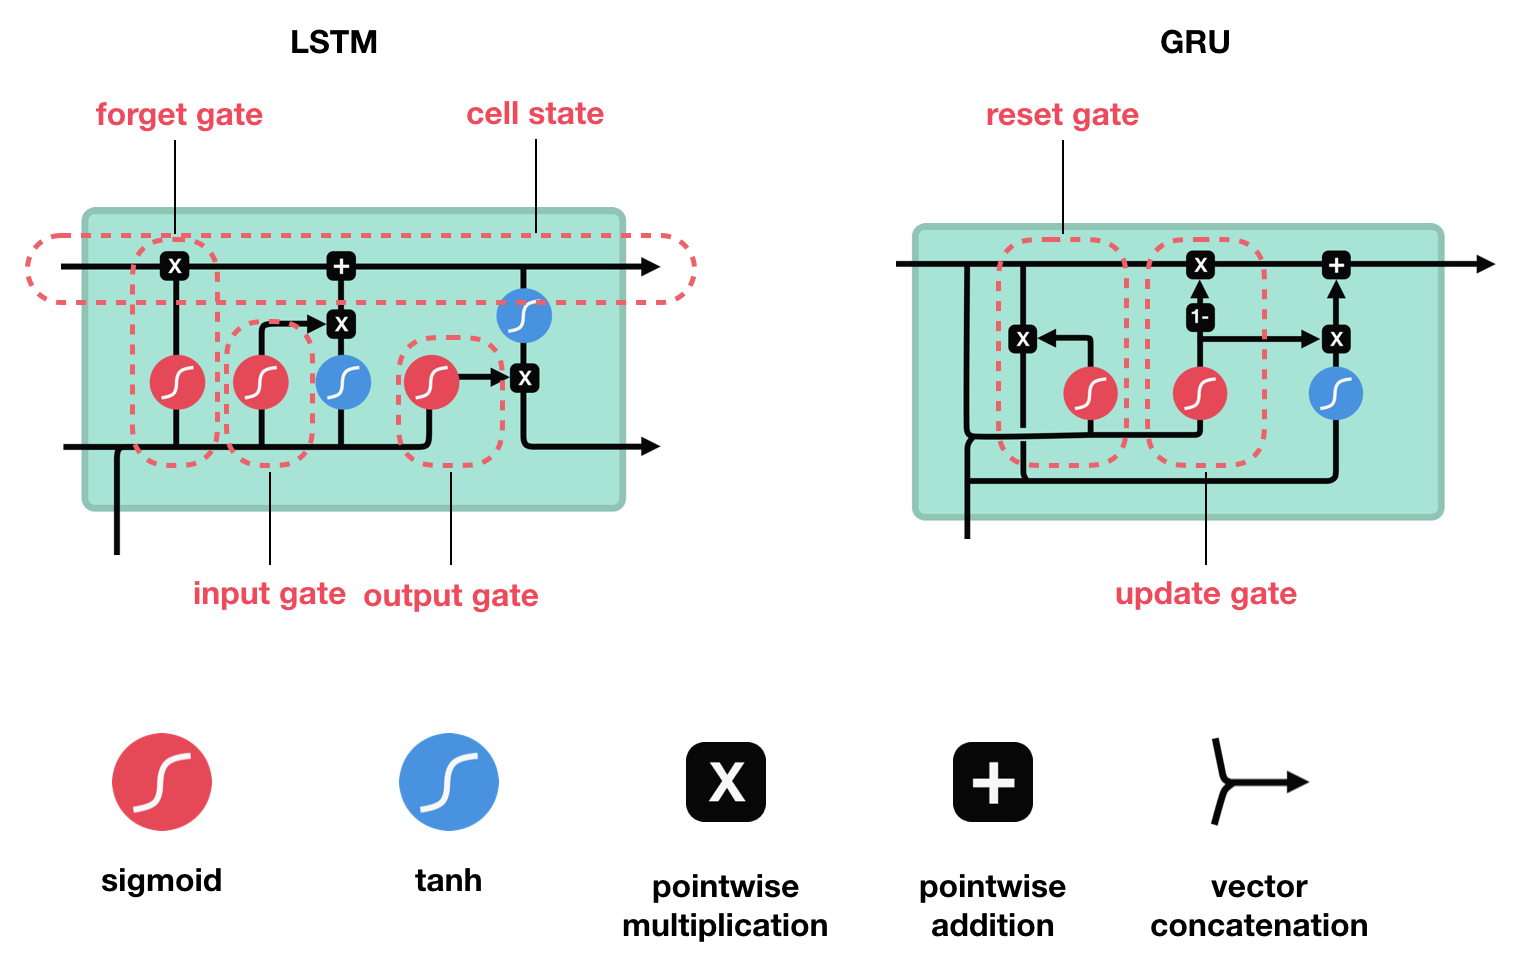
\includegraphics[width=0.84\textwidth]{images/arte/lstmvsgru}
	\caption{Arquitectura celdas LSTM y GRU. Fuente \cite{lstmgru}}
	\label{fig:lstmvsgru}
\end{figure}



Debido al éxito de las celdas LSTM, y al constante esfuerzo de optimización de las mismas, han surgido diferentes variantes. La más conocida de todas son las \textit{Gated Recurrent Unit} (\textbf{GRU}) introducidas en 2014. La celda GRU es una simplificación de la celda LSTM y produce unos rendimientos bastante similares con un menor coste. De manera muy resumida una celda GRU se compone de: 
\begin{itemize}
	\item Puerta de reset: Permite seleccionar que información de la memoria va a ser utilizada en un paso concreto. 
	\item Puerta de actualización: Realiza la función de las puertas de olvido y de entrada que hemos visto en las celdas LSTM.
\end{itemize}

Aunque no hemos entrado en el detalle del funcionamiento de cada una de las puertas, en la Figura \ref{fig:lstmvsgru} podemos ver la arquitectura completa de ambos tipos, y observar la mayor simplicidad de las celdas GRU frente a las LSTM. 


Como podemos imaginar, las redes neuronales recurrentes son ampliamente usadas en el mundo del Procesamiento del Lenguaje Natural, debido a que una palabra no es otra cosa que una secuencia de letras, una frase a su vez se trata de una secuencia de palabras y un documento una secuencia de frases. Alguno de los usos de las RNN en este ámbito son: 

\begin{itemize}
	\item \textbf{Análisis de sentimientos}: Detectar el sentimiento positivo o negativo de un texto utilizando únicamente la última salida de la red. En \cite{rnnej1} tenemos un ejemplo de análisis de sentimientos utilizando redes recurrentes con LSTM sobre los datos de una red social China.
	\item \textbf{Generador de texto}: Predecir la siguiente palabra de una secuencia, utilizando la salida de cada una de las celdas. Podemos ver una comparación de métodos para generar textos de diferentes temáticas para poder entrenar posteriormente modelos \textit{Deep Learning} en \cite{rnnej2}. Entre los métodos de la comparación se encuentran las redes neuronales recurrentes con celdas GRU y con celdas LSTM.
	\item \textbf{Traductores}: Traducción automática de textos entre idiomas, llamado \textit{Neural Machine Translation} (NMT) cuando se utilizan redes neuronales.  Quizás el mayor caso de éxito en este punto es el \textit{Google's Neural Machine Translation System} \cite{rnnej3} cuya base es una red neuronal profunda construida con celdas LSTM.
\end{itemize}



Una vez analizadas, de manera global, las redes neuronales recurrentes podemos ver que nos ofrecen \textbf{numerosas ventajas al trabajar con secuencias} como hacemos en el ámbito del PLN. Entre ellas podemos ver, que vamos incluso más allá que con las CNN analizando la relación entre las diferentes palabras, fundamentalmente con las celdas LSTM y GRU, pudiendo detectarlas entre palabras que estén alejadas entre sí y no ceñirnos al tamaño del kernel. Sin embargo, como hemos visto, y aunque sean mitigados por el uso de celdas LSTM y GRU, las redes neuronales recurrentes presentan \textbf{problemas durante el entrenamiento} tanto de desvanecimiento como de explosión del gradiente.


\section{\textit{BigData} y \textit{Fast Data}}
\label{section:arte:big}
A lo largo de esta sección intentaremos tener una visión general del \textit{Big Data} y su evolución a lo largo del tiempo hasta llegar al \textit{Fast Data}. Posteriormente veremos las arquitecturas más usadas en el mundo del \textit{Big Data}. 

\subsection{Evolución: del \textit{Big Data} al \textit{Fast Data}}

El primer uso del término  \textit{Big Data}  se da en un artículo de Michael Cox y David Ellsworth de la NASA publicado en 1997 \cite{Cox_1997}, donde hacen referencia a la dificultad de procesar grandes volúmenes de datos con los métodos de la época. Sin embargo, fue en 2001 cuando encontramos la definición más conocida y aceptada de \textit{Big Data} hecha por el analista Laney Douglas en su artículo ``\textit{3D Data Management: Controlling Data Volume, Velocity y Variety}'' \cite{laneay_2013} en el que se hacía referencia a las ya ``famosas'' tres \textit{V}s:

\begin{itemize}
	\item \textbf{V}olumen:  Cada vez los volúmenes de datos son mayores.
	\item \textbf{V}elocidad: Es cada vez mayor la velocidad con la que se generan los datos.  
	\item \textbf{V}ariedad: Dejamos de tener únicamente datos completamente estructurados para trabajar con datos no estructurados y/o  semi-estructurados. 
\end{itemize} 


Google, como es obvio, también  se enfrentó a un importante problema a la hora de procesar la ingente cantidad de datos que generaba día a día y que no podían ser procesados de manera eficiente con el \textit{software} existente, es por ello que en el año 2003 presenta en \cite{GFS} su  \textit{``Google File System''} (GFS) y un año después \textit{Map Reduce} \cite{MapReduce}, estas dos capas de almacenamiento y procesamiento distribuido dieron lugar al nacimiento de lo que hoy conocemos como \textit{\textbf{Big Data}}.

Sin embargo, estas aportaciones no empezaron a tomar una repercusión relevante fuera de Google hasta el nacimiento del \textit{framework} Hadoop en 2006, un ecosistema con una gran cantidad de servicios pero cuya base fue Map Reduce y HDFS (basado en GFS). La complejidad del ecosistema \textit{Hadoop} hizo que éste no empezara a aparecer en la mayoría de las empresas hasta la creación de la compañía \textit{Cloudera} en 2009, que empezó a empaquetar los diferentes componentes del ecosistema \textit{Hadoop}, ofreciendo distribuciones estables y soporte para sus clientes. 


\begin{figure}[!ht]
	\centering
	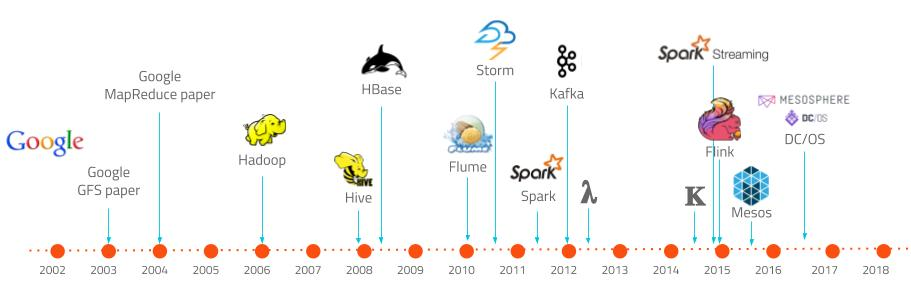
\includegraphics[width=0.94\textwidth]{images/arte/bigdatatime}
	\caption{Evolución del \textit{Big Data}. Fuente \cite{lambdakappa}}
	\label{fig:bigdatatime}
\end{figure}


Durante estos 10 años la popularidad de \textit{Hadoop} ha crecido exponencialmente y junto con las BBDD NoSQL, nacidas también a partir de Google con su BigTable, forman lo que hoy conocemos como Big Data. En la Figura \ref{fig:bigdatatime} observamos esta evolución en el mundo del \textit{Big Data} con los hitos de aparición de algunas tecnologías representativas.



El auge del \textbf{Big Data} ha llevado a algunas empresas a tener verdadera obsesión por el almacenamiento de todos los datos de sus clientes y las operaciones realizadas, creando inmensos \textit{datalakes} donde tener enormes históricos de todos sus datos. Este ``síndrome de Diógenes digital'' creado por falsas expectativas, por la imposibilidad de extraer valor de los datos o por la dimensión cambiante de las empresas actuales (en la que los datos de años atrás pueden no ser relevantes en el presente), es uno de los posibles motivos por lo que el tratamiento de los datos esta cambiando. Otro de los motivos para el cambio de rumbo del \textit{Big Data} está relacionado con la \textit{V} de Velocidad, hoy en día no solo es importante la capacidad de ingestar rápidamente los datos, sino la capacidad de poder procesar y obtener decisiones o actuar en tiempo real a partir de los datos, aportando valor al negocio. En este escenario se vuelve más importante la velocidad que el volumen de datos, esto es lo que se denomina \textit{Fast Data}. 



Dentro del \textit{Fast Data} es habitual el uso de BBDD \textit{in-memory}, de buses de eventos y de tecnologías de procesamiento capaces de procesar los eventos en tiempo real. Como veremos posteriormente al desarrollar nuestra arquitectura, el \textit{Fast Data} será una parte fundamental en nuestro proyecto en el que tendremos que clasificar las llamadas en tiempo real y tomar decisiones (o alarmar) en función de las mismas. 

Observando de nuevo la Figura \ref{fig:bigdatatime} podemos ver este cambio en la tendencia hacia el \textit{Fast Data} a partir del 2012 cuando aparece la tecnología Kafka y en los años posteriores con la incorporación de diferentes herramientas para el procesamiento de eventos como son \textit{Spark Streaming} o \textit{Flink}.

\subsection{Arquitecturas \textit{RealTime}}
La evolución que hemos visto en el apartado anterior,  con la explosión del \textit{Big Data} y la irrupción del \textit{Fast Data}, hace necesaria la incorporación en las empresas de arquitecturas de procesamiento de datos en tiempo real que, como cualquier otra arquitectura de datos, sean capaces de ingestar, procesar y permitir la explotación y análisis de los datos. La diferencia fundamental en las arquitecturas \textit{RealTime} y las arquitecturas de datos tradicionales son el\textbf{ volumen de los datos a tratar} y la \textbf{capacidad para hacerlo en tiempo real}.

Como veremos, no existe una arquitectura que se adapte a todos los casos de uso (\textit{one-size-fits-all}) y, según la necesidad, será necesario aplicar una u otra.

\subsubsection{Arquitectura Lambda $\lambda$}
La arquitectura lambda, representada por la letra griega $\lambda$, fue presentada en 2011 por Nathan Marz en un artículo publicado en su blog titulado ``\textit{How to beat the CAP theorem}'' \cite{lambda}.

\begin{figure}[!ht]
	\centering
	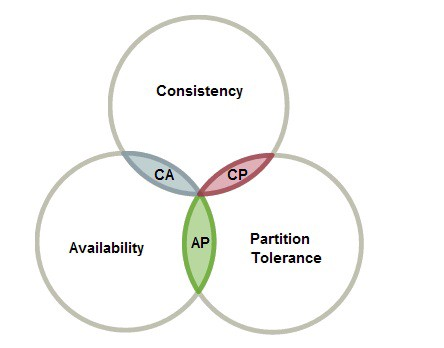
\includegraphics[width=0.55\textwidth]{images/arte/cap}
	\caption{Teorema CAP. Fuente \cite{cap}}
	\label{fig:cap}
\end{figure}

El propósito de Nathan Marz cuando crea su arquitectura, como indica el título del artículo, es batir el teorema CAP popularizado por la irrupción de las bases de datos NoSQL. Este teorema, ilustrado en la Figura \ref{fig:cap}, viene a decir que si queremos tener tolerancia a particiones (imprescindible para bases de datos distribuidas necesarias para el \textit{Big Data}), tenemos que optar entre consistencia, asegurar que el dato que leemos es el último que hemos escrito, o disponibilidad, que la base de datos se encuentra siempre lista.



El método propuesto para conseguir este objetivo con grandes cantidades de datos se basa en los siguientes principios:

\begin{itemize}
	\item Una capa \textit{batch} eventualmente consistente de una manera extrema, en la que las escrituras tardan siempre unas pocas horas en estar disponibles. Eliminando algunos problemas complejos con los que tratar como  la concurrencia o las reparaciones de lectura. 
	\item Reducir las operaciones CRUD (\textit{\textbf{C}reated, \textbf{R}ead, \textbf{U}pdate, \textbf{D}elete}) en la capa \textit{batch} por únicamente CR, tratando los datos como objetos inmutables. Esto nos soluciona el problema de la consistencia, ya que de este modo un dato existe o no existe, pero no puede tener varias versiones. 
	\item Una capa \textit{realtime} que se encarga de los datos de las últimas horas (los que no están disponibles en la capa \textit{batch})
	\item Las querys atacan a ambas capas de forma simultanea realizando un \textit{merge} de los datos.
	
\end{itemize}

\begin{figure}[!ht]
	\centering
	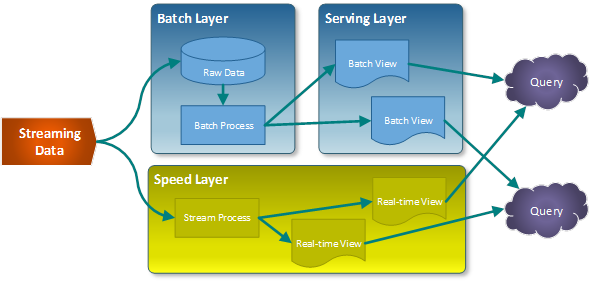
\includegraphics[width=0.70\textwidth]{images/arte/lambda}
	\caption{Arquitectura Lambda definida por   Nathan Marz. Fuente \cite{lambdakappa}}
	\label{fig:lambda}
\end{figure}


Podemos ver un esquema de la arquitectura en la Figura \ref{fig:lambda}. Esta arquitectura, aparte de resolver los problemas de consistencia y disponibilidad, tiene algunas ventajas:

\begin{itemize}
	
	\item Disponer de todos los datos en un único punto (capa \textit{batch}) pudiendo realizar cualquier tipo de consulta sobre los mismos. 
	\item Al utilizar los datos como un ente inmutable facilita las auditorias. 
	\item Según Marz, evita el error humano en la capa \textit{batch} (en parte también por usar datos inmutables), y cualquier error en la capa \textit{realtime} sería subsanado en pocas horas en la capa \textit{batch}.

\end{itemize}


\subsubsection{Arquitectura Kappa $\kappa$}  
En su artículo ``Questioning the Lambda Architecture''\cite{kappa}, Jay Kreps cuestiona la arquitectura Lambda propuesta por Nathan Marz y propone una simplificación de la misma, basada en su experiencia en LinkedIn trabajando con Kafka y Samza. Esta simplificación se denomina arquitectura Kappa y viene representada por la letra griega $\kappa$.


Kreps describe la complejidad que supone en una arquitectura Lambda mantener idénticos procesos en \textit{realtime} y \textit{batch}. También expone que se menosprecia la capacidad de la capa \textit{realtime} (probablemente por la madurez del procesamiento \textit{realtime} con respecto al \textit{bacth}) y opina que es posible realizar el mismo procesamiento, incluso reprocesar el histórico de datos, en la capa \textit{realtime}. 

\begin{figure}[!ht]
	\centering
	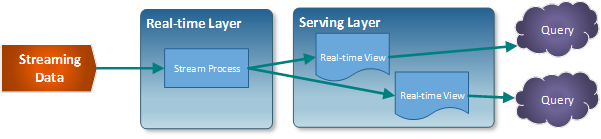
\includegraphics[width=0.70\textwidth]{images/arte/kappa}
	\caption{Arquitectura Kappa definida por Jay Kreps. Fuente \cite{lambdakappa}}
	\label{fig:kappa}
\end{figure}

Con esta premisa, en el artículo se presenta la arquitectura que observamos en la Figura \ref{fig:kappa}, en la que existe un único flujo de procesamiento \textit{realtime} para todo el modelo. La simplicidad de Kappa con respecto a Lambda es tal que el propio Kreps afirma que puede ser una idea demasiado simple para merecer una letra griega.



\section{Trabajos anteriores}
\label{section:arte:ant}


Una vez abordado el estado del arte desde diferentes puntos de vista, es importante tener una visión de los trabajos anteriores que se han realizado con objetivos similares y sus resultados. De este modo entenderemos si existe una justificación para nuestro trabajo, los problemas a los que podemos enfrentarnos y las expectativas que podemos gestionar.

En este apartado nos vamos a  centrar en la aplicación de técnicas de Procesamiento del Lenguaje Natural a un \textit{Call Center}. Encontramos varios artículos interesantes que hacen hincapié en el valor de la información y el conocimiento que puede extraerse de un \textit{Call Center}, ya que se trata de un intermediario importante entre el cliente y la empresa. Entre estos trabajos podemos destacar: 

\begin{itemize}
	\item ``Metodología para estimar el impacto que generan las llamadas realizadas en un call center en la fuga de los clientes utilizando técnicas de text mining'' \cite{call1}: Que como su nombre indica, investiga si existe relación entre las llamadas realizadas al \textit{Call Center} y la pérdida de clientes. El trabajo, al igual que el proyecto que intentamos abordar, parte de las llamadas transcritas a texto y, aunque se utiliza como base para la modelización de temas LDA, se apoya en etiquetas existentes en las llamadas para validar los resultados.
	
	\item ``Customer voice sensor: A comprehensive opinion mining system for call center conversation'' \cite{call2}: Se trata de un trabajo más basado en el análisis de sentimientos, pero se encuentra realizado con llamadas de los clientes a una operadora de telecomunicaciones (en este caso China Telecom) al igual que nuestra fuente de información.
	
	\item ``Topic mining for call centers based on A‐LDA and distributed computing'' \cite{call3}: En este caso, se realiza una modelización de temas sobre  los datos del \textit{Call Center} de \textit{China Central Television}. En este proceso de modelización se utiliza  una mejora del modelo LDA llamada A-LDA que utiliza no solo el corpus de la llamada, si no también algunas propiedades externas como el tiempo de llamada o el número de origen.
	
	\item ``Author-topic based representation of call-center conversations'' \cite{call4}: Este último artículo que comentamos, parte también de los datos generados a través de un \textit{Performance of Automatic Speech Recognition} (ASR), el trabajo pone de manifiesto la pobre calidad de estas transcripciones automáticas. Por este motivo, propone una modificación de LDA basada en el modelo \textit{Author Topic}, utilizando además del corpus del texto información del tema de la conversación.
\end{itemize}


Probablemente, dentro de las empresas, existen muchos más trabajos destinados a la explotación de esta información y que no se encuentren publicados, por lo que podemos concluir que es un campo que despierta interés y que se trata de una información con potencial que nos permita, entre otros objetivos, comprender las necesidades de los clientes de una compañía.

Por otro lado, observamos que en la mayoría de los casos, aunque la base de la modelización sea el uso de LDA, debido al ruido o a otros factores como la ausencia de información semántica, se utilizan modificaciones del modelo que incorporan etiquetas o propiedades externas al corpus para mejorar la clasificación.

Por último, pensamos que, aún con estos antecedentes, existe la necesidad de abordar este proyecto, debido a la diferencia entre unos datos y otros, por factores como el idioma o las distintas necesidades de cada empresa. Además nuestro proyecto tiene como objetivo final la integración de este modelo en un proceso de la compañía que sea capaz de aplicarlo en tiempo real y alertar en caso de anomalías para poder tomar decisiones.

